\section{Results and Discussion}
\label{sec:results}

In this thesis we have presented a measurement of the $\nu_\mu$ induced flux-averaged, charged current inclusive, absolute cross section on water. We use data from all four beam run periods with an accumulated exposure of 5.636$\times 10^{20}$ protons on target. Charged current inclusive events are selected in the water target volume of the P0D by requiring the produced muon to pass through the Tracker that is directly downstream. Data is collected from the P0D while it is both filled with water and drained of water. The background contamination and the signal efficiency are both estimated using NEUT MC. After background subtracting and efficiency correcting the water-in and water-out CC inclusive event rates, we perform a statistical subtraction to extract the absolute water cross section.

There are several detector level corrections that are made. Specifically, the MC estimations for background and signal efficiency are corrected for small differences between data and MC in the P0D fiducial mass, the track matching efficiency, and the sand muon interference rate. These corrections shift the central value of the absolute water cross section by a small amount. Many sources of systematic uncertainty have also been evaluated. These include the flux systematic uncertainty, the standard interaction cross section model uncertainty, the final state interaction cross section model uncertainty and a host of detector level systematic uncertainties. Fractionally, the flux, physics model and detector systematic uncertainties are $^{-9.62\%}_{+11.09\%}$, $^{-13.43\%}_{+8.79\%}$ and $\pm 2.02\%$ respectively. This yields a total systematic uncertainty of $-16.64\%$ and $+14.29\%$ fractionally.

As our analysis studies charged current interactions and we do not distinguish interactions on protons and neutrons, our result is a cross section measurement per nucleon. However, water is not an iso-scalar target, so the result is given per H$_2$O nucleon. We also include a result per water molecule. The final, $\nu_\mu$ induced, flux-averaged CC inclusive absolute water cross section is:

\begin{equation}
\left<\sigma\right>_\Phi = (6.37 \pm 0.157 (stat.) ^{-1.060}_{+.910} (sys.))\times 10^{-39} \frac{\text{cm}^2}{H_2O\:\text{nucleon}}
\end{equation}

\begin{equation}
\left<\sigma\right>_\Phi = (11.5 \pm 0.284 (stat.) ^{-1.91}_{+1.64} (sys.))\times 10^{-38} \frac{\text{cm}^2}{H_2O\:\text{molecule}}
\end{equation}

To compare to other results from different neutrino experiments, it is useful to convert our cross section measurement to that on an iso-scalar target such as carbon. The inclusive charged current cross section of a neutrino with a neutron has been observed to be higher than that of a neutrino with a proton. An iso-scalar target has the same number of neutrons and protons, so to compare to such a target, we must average out the structure of our own nucleus. In water, there are 10 protons and 8 neutrons, so we use the following correction formula:

\begin{equation}
\left<\sigma\right>_\Phi^{iso} = \left<\sigma\right>_\Phi^{H_2O}*\frac{(10\sigma(\nu p)+8\sigma(\nu n))/18}{(\sigma(\nu p)+\sigma(\nu n))/2}
\end{equation}
where $\sigma(\nu p)$ and $\sigma(\nu n)$ are the CC inclusive cross sections on protons and neutrons individually. We use a  $\sigma(\nu n)/\sigma(\nu p)$ ratio of 3.3 to calculate the corrected cross section per iso-scalar nucleon for comparison. The value of 3.3 was extracted from a digitized plot of the BNL-7ft experiment results that measure the relative neutron and proton cross sections. Note that as we expect some coherent neutrino interactions, this iso-scalar conversion does not account for nuclear effects.

The $\nu_\mu$ induced, flux-averaged CC inclusive absolute water cross section per iso-scalar nucleon is:

\begin{equation}
\left<\sigma\right>_\Phi^{iso} = (6.77 \pm 0.167 (stat.) ^{-1.127}_{+.968} (sys.))\times 10^{-39} \frac{\text{cm}^2}{\text{iso. nucleon}}.
\end{equation}
This result can be compared to the result from Ref\cite{ccinc} that used the Tracker for a similar CC inclusive selection on primarily carbon which is an iso-sclar target. The analysis in Ref\cite{ccinc} has a higher efficiency of high-angle and low momentum muon tracks. They find a flux averaged CC inclusive cross section of $(6.93 \pm 0.13 (stat.) \pm 0.85(sys.)) \times 10^{-39} \frac{cm^2}{nucleons}$. These results are quite compatible as we would expect. Note that the flux and model systematics are very highy correlated between these two measurements. We can also compare our iso-scalar result with the NEUT and GENIE predictions in Ref\cite{ccinc}. They predict that the cross sections are:

\begin{equation}
\left<\sigma\right>_\Phi^{NEUT} = 7.26 \times 10^{-39} \frac{cm^2}{nucleon}
\end{equation}

\begin{equation}
\left<\sigma\right>_\Phi^{GENIE} = 6.68 \times 10^{-39} \frac{cm^2}{nucleon}
\end{equation}

For comparison with other data, we present our result and the NEUT/GENIE predictions as a cross section per GeV. The P0D T2K result is shown in figure \ref{fig:xsdata} overlaid on results from several other experiments. The colored lines show the NEUT and GENIE predictions for T2K as extracted from Ref \cite{ccinc}. Some of the data were digitized directly from the relevant publications and others were taken from tables or data releases. We have marked the data sets that were collected through digitization in the figure. Furthermore, many results were quoted as an absolute cross section instead of cross section divided by neutrino energy. We took a direct division of the cross section and the mean neutrino energy without adding any neutrino energy shape errors to the systematic envelope of the divided result. The neutrino energy shape errors should be accounted for in the horizontal error bars. Finally, for a few data points, we do not show a horizontal error bar. This is either a result of no horizontal errors being provided or no meaningful digitization of horizontal error bars being available in the publications. In our case, it is a nontrivial matter to calculate an error envelope on the neutrino flux. We do not provide one in this plot. For the mean neutrino energy of T2K, we use the value of 0.85~GeV \cite{ccinc}.

We find that our error bars are comparable to the most precise measurements of neutrino cross section at such low energies. We are also consistent with global data and the GENIE cross section prediction. We are also the very first inclusive charged current cross section result on the non-isoscalar target of water, a common target in many neutrino detectors. In the future, we can hope to extract the ratios of exclusive neutrino interactions and to compare nuclear effects on a water molecule. We can also, with better reconstruction techniques, achieve higher efficiencies at steeper muon angles and lower neutrino energies. Finally, with the proper treatment of migration errors, it is also possible to extend this result into multiple bins of muon kinematic observables to extract a single or double differential cross section on water.
\afterpage{
\begin{landscape}
\begin{figure}[h]
\centering
$\vcenter{\hbox{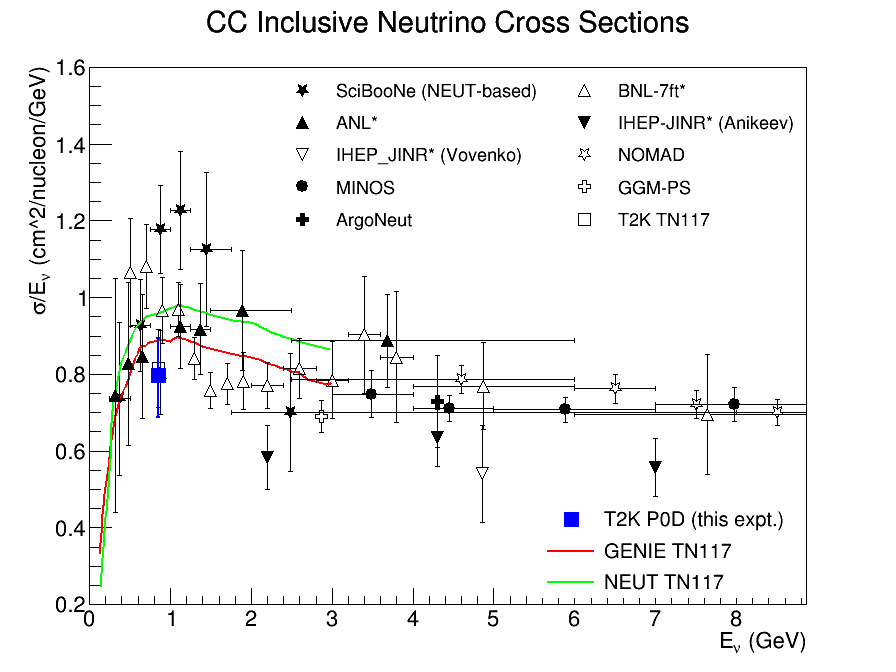
\includegraphics[height=5.5in]{Figures/XSec.png}}}$
\caption{Absolute neutrino cross sections divided by mean neutrino energy for various experiments. The result from this analysis is shown in blue with total vertical error bars. No error on the mean neutrino energy is shown. Experiment names marked with (*) have data extracted from plots by digitization. The MC predictions are taken directly from digitizing the NEUT/GENIE figure from Ref\cite{ccinc}.}
\label{fig:xsdata}
\end{figure}
\end{landscape}
}